\section{Tấn công từ chối dịch vụ (DoS) và tấn công từ chối dịch vụ phân tán (DDoS)}

\subsection{Tấn công từ chối dịch vụ}

\subsubsection{Tấn công từ chối dịch vụ là gì?}

Theo định nghĩa của \cite{1-dos-concept}, một cuộc tấn công từ chối dịch vụ diễn ra khi người dùng hợp lệ không có khả năng truy cập thông tin từ các hệ thống, các thiết bị hoặc các tài nguyên mạng do sự can thiệp của nhân tố mạng độc hại. Những dịch vụ bị ảnh hưởng bao gồm thư điện tử, các trang mạng, các tài khoản trực tuyến (ví dụ như ngân hàng), hay các dịch vụ khác dựa trên tài nguyên máy tính hoặc tài nguyên mạng. Tình trạng ''từ chối dịch vụ''  là khi hệ thống hay mạng lưới của nạn nhân bị làm ngập lụt cho đến lúc không còn khả năng phản hồi, sụp đổ, hay ngăn chặn sự truy cập từ những người dùng hợp lệ. Tấn công từ chối dịch vụ có thể gây hại cho các tổ chức cả về tiền bạc lẫn thời gian trong lúc dịch vụ của họ không thể truy cập được.

Có rất nhiều phương thức để thực hiện tấn công DoS. Phương thức thông thường diễn ra là khi kẻ tấn công làm ngập lụt mạng lưới hệ thống với lưu lượng. Với phương thức này, kẻ tấn công gửi hàng loạt yêu cầu đến máy chủ nạn nhân, làm cho nó quá tải. Những yêu cầu dịch vụ này là bất hợp lệ và có địa chỉ giả mạo, sẽ gây nhầm lẫn cho máy chủ khi nó cố gắng xác thực người gửi yêu cầu. Khi những yêu cầu thừa thải được xử lý liên tục, máy chủ sẽ bị quá tải, từ đó tạo nên trạng thái từ chối dịch vụ đối với các yêu cầu hợp lệ.

\subsubsection{Những loại tấn công DoS thường gặp}

Trong tấn công Smurf \cite{1-dos-concept}, những kẻ tấn công gửi các gói tin broadcast ICMP đến một số lượng đáng kể các máy chủ với các địa chỉ IP nguồn giả mạo, thứ thuộc về máy chủ nạn nhân. Các máy chủ nhận những gói tin này sẽ phản hồi và từ đó làm ngập lụt máy chủ nạn nhân với những gói tin phản hồi này.

Tấn công ngập lụt gói tin SYN \cite{1-dos-concept} diễn ra khi một kẻ tấn công gửi một yêu cầu để kết nối đến máy chủ nạn nhân nhưng lại không hoàn thành kết nối đó thông qua việc bắt tay ba bước – một phương thức được dùng trong mạng lưới TCP/IP để tạo kết nối giữa máy chủ và máy khách. Việc không hoàn thành kết nối sẽ dẫn tới cổng kết nối giữ trạng thái ''bị chiếm giữ'' và không khả dụng cho các kết nối sau này. Kẻ tấn công cứ liên tiếp tạo các kết nối, chiếm giữ tất cả các cổng và từ đó ngăn chặn những người dùng hợp lệ có thể tạo các kết nối mới.

Những mạng lưới cá nhân có thể bị ảnh hưởng bởi các tấn công DoS mà không phải là mục tiêu trực tiếp. Nếu nhà cung cấp dịch vụ Internet hoặc nhà cung cấp dịch vụ đám mây bị nhắm đến và bị tấn công, thì mạng lưới cũng sẽ trải qua việc mất dịch vụ.

Tấn công ngập lụt UDP \cite{2-imperva} diễn ra dựa trên sự không tin cậy của kết nối UDP. Trong tấn công này, rất nhiều gói tin UDP với các cổng ngẫu nhiên được gửi tới nạn nhân. Khi nạn nhân nhận gói tin tại một cổng, nó sẽ tìm kiếm ứng dụng đang lắng nghe cổng đó. Khi nó không tìm được, nó sẽ phản hồi với một gói tin ICMP báo lỗi. Khi một lượng lớn gói tin UDP độc hại được nhận, nạn nhân sẽ tiêu thụ rất nhiều tài nguyên trong việc phản hồi với các gói tin ICMP. Điều này sẽ ngăn chặn nạn nhân phản hồi những người dùng hợp lệ.
 
Slowris \cite{2-imperva} là loại tấn công cho phép một máy tính làm sập các máy chủ web chỉ với một lượng băng thông nhỏ nhưng lại không ảnh hưởng đến các dịch vụ khác của nạn nhân. Slowris thực hiện việc này bằng cách giữ càng nhiều kết nối đến máy chủ web nạn nhân càng lâu càng tốt. Nó sẽ tạo kết nối đến với máy chủ web nạn nhân, tuy nhiên nó chỉ gửi một phần của yêu cầu. Nó liên tục gửi các HTTP header nhưng không bao giờ hoàn thành chúng. Nạn nhân sẽ liên tục giữ những kết nối độc hại này được mở, từ đó dẫn đến quá tải giới hạn kết nối, dẫn đến việc từ chối dịch vụ tới các người dùng hợp lệ.

\subsection{Tấn công từ chối dịch vụ phân tán}

\subsubsection{Tấn công từ chối dịch vụ phân tán là gì?}

Có rất nhiều định nghĩa tấn công DDoS từ các nghiên cứu khác nhau, tuy nhiên chung quy đều có chung suy nghĩ và ý nghĩa.
Theo như \cite{1-dos-concept}, tấn công từ chối dịch vụ diễn ra khi nhiều máy tính vận hành cùng lúc với nhau để tấn công vào một mục tiêu. Những kẻ tấn công thường tận dụng mạng lưới Botnet – một nhóm các thiết bị truy cập Internet bị chiếm giữ - để dẫn tới một tấn công quy mô lớn. Những kẻ tấn công sẽ tìm kiếm và chiếm giữa  các mạng lưới hay thiết bị kết nối Internet có bảo mật kém, từ đó tạo nên mạng Botnet. Tấn công DDoS tạo một lượng yêu cầu cực lớn đến nạn nhân, từ đó gia tăng sức mạnh tấn công, đồng thời rất khó để phòng thủ bởi tính đa dạng và rộng khắp từ các nguồn tấn công.

Nam-Seok Ko và các cộng sự \cite{3-Ko} giải thích rằng tấn công DDoS là sự kết hợp của việc sử dụng một lượng cực lớn lưu lượng mạng bởi kẻ tấn công nhắm vào hệ thống mục tiêu thông qua việc vận hành đồng thời một lượng lớn máy tính được phân tán trên Internet. Theo như nghiên cứu này, lưu lượng tấn công sẽ ngăn cản người dùng thực tế truy cập vào tài nguyên của nạn nhân bằng việc thâu tóm tất cả băng thông mạng và tài nguyên bên trong hệ thống.

Fallah và các cộng sự \cite{4-Fallah} thì cho rằng, tấn công DDoS bắt đầu bằng việc kẻ tấn công sẽ truy tìm các máy chủ có các lỗi bảo mật trên Internet, để có thể xâm nhập và điều khiển chúng gửi một lượng lớn các gói tin đến máy chủ nạn nhân. Hơn nữa, khi kẻ tấn công thành công, chúng đã có thể sử dụng toàn bộ tài nguyên máy chủ như CPU, stack space trong giao thức phần mềm, hoặc Internet link capacity, từ đó nạn nhân không thể cung cấp dịch vụ đến với người dùng thực tế của nó.

Từ góc nhìn của doanh nghiệp, Yoon \cite{5-Yoon} giải thích rằng tấn công DDoS được thể hiện bằng việc kẻ tấn công bên ngoài trên Internet sử dụng BotMaster điều khiển từ xa các Botnet nhằm thực hiện tấn công vào các trang web quan trọng từ đó các dịch vụ kinh doanh thiết yếu như Internet banking, e-government, e-trading, e-commerce, vv, bị vô hiệu hóa đối với người dùng.

Theo \cite{1-dos-concept}, các cuộc tấn công DDoS đã gia tăng cường độ khi ngày càng có nhiều thiết bị IoT ra đời. Các thiết bị IoT thường sử dụng mật khẩu mặc định và không được bảo mật kỹ càng khiến chúng rất dễ bị xâm nhập và khai thác. Việc lây nhiễm các thiết bị IoT thường không được nhiều người chú ý, kẻ tấn công có thể xâm nhập và điều khiển hàng trăm nghìn thiết bị IoT, từ đó thực hiện một cuộc tấn công DDoS quy mô lớn mà người sở hữu thiết bị không hay biết hề hay biết.

Trên thực tế hiện nay, mặc cho các cuộc tấn công DDoS rất khó ngăn chặn và giảm thiểu thiệt hại thì vẫn chưa có một phương thức phòng chống tiêu chuẩn nào được đưa ra. Điều này phần lớn là do DDoS cố gắng bắt chước lưu lượng thông thường nhưng với mật độ yêu cầu khổng lồ.

Mô hình tấn công DDoS được mô tả như trong hình \ref{fig:ddos-model-example}.

\begin{figure}[ht!]
	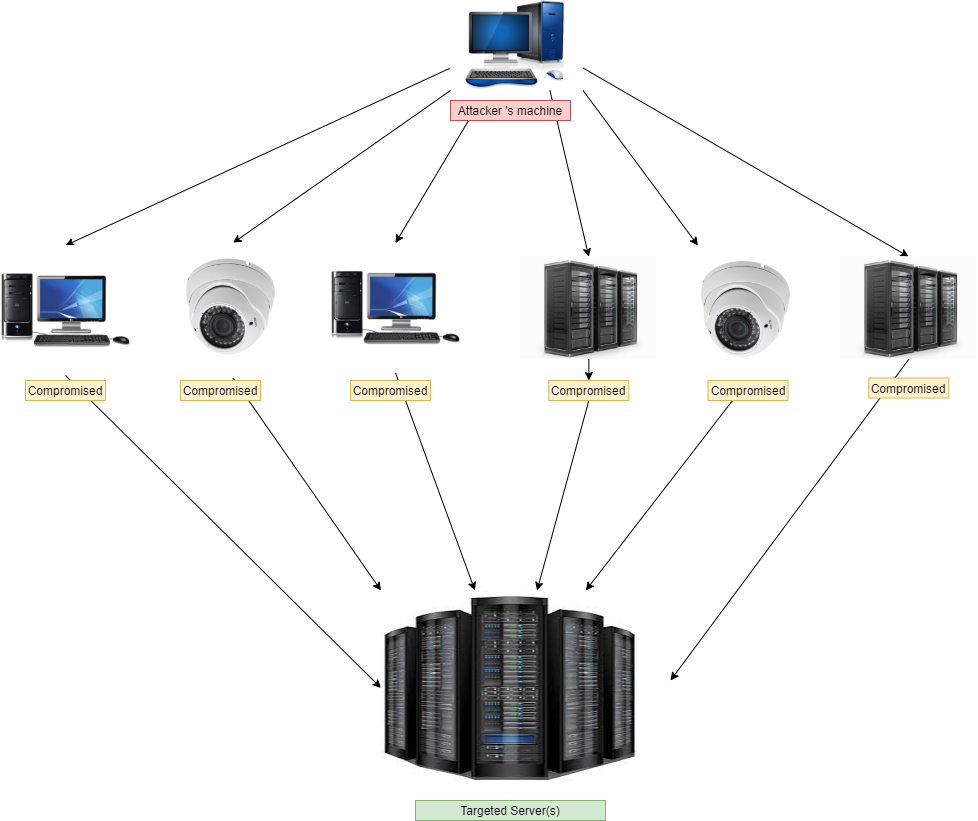
\includegraphics[width=\linewidth]{fig/ddos-model-example.png}
	\caption{Mô hình tấn công DDoS}
	\label{fig:ddos-model-example}
\end{figure}

\subsubsection{Các loại tấn công từ chối địch vụ phân tán thường gặp}

Nhìn chung, theo như các định nghĩa thì tấn công DDoS được thực hiện khi có rất nhiều thiết bị cùng lúc thực hiện tấn công DoS. Một số loại tấn công DDoS có thể liệt kê như sau:

Tấn công khuếch đại NTP \cite{2-imperva}, kẻ tấn công sẽ khai thác những máy chủ NTP công khai để làm quá tải nạn nhân với lưu lượng UDP. Loại tấn công này được xem là tấn công khuếch đại cưỡng đoạt bởi vì tỷ lệ phản hồi trong kịch bản này nằm ở đoạn 1:20 đến 1:200 và hơn thế nữa. Điều này có nghĩa là một kẻ tấn công nắm một lượng lớn máy chủ NTP có thể dễ dàng tạo nên tấn công DDoS với băng thông và lưu lượng cực lớn.

Tấn công ngập lụt HTTP \cite{2-imperva} là loại tấn công mà kẻ tấn công sẽ gửi những yêu cầu GET/POST HTTP trông giống các yêu cầu hợp lệ tới máy chủ web hoặc ứng dụng. Tấn công này không gửi các gói tin dị thường, kỹ thuật giả mạo hay phản chiếu, và yêu cầu ít băng thông hơn các kiểu tấn công khác để làm sập máy chủ nạn nhân. Đây là loại tấn công hiệu quả nhất khi nó buộc máy chủ hay ứng dụng phải sử dụng tối đa tài nguyên cho mỗi yêu cầu.

\subsubsection{Các đợt tấn công DoS/DDoS điển hình}

Theo \cite{6-wired} ghi nhận, vào năm 2016 thế giới chứng kiến một đợt tấn công DDoS ''lớn nhất từ trước đến nay'' nhắm vào Dyn – một đơn vị cung cấp dịch vụ DNS của Hoa Kỳ. Cuộc tấn công này là hệ quả từ việc bảo mật yếu kém từ các thiết bị IoT, cho phép kẻ tấn công chiếm quyền kiểm soát và cài đặt botnet. Đỉnh điểm của cuộc tấn công lên đến 1.2Tbps.

Theo \cite{7-wired}, vào năm 2018, Github – một công ty cung cấp dịch vụ lưu trữ mã nguồn lớn nhất thế giới có trụ sở tại Hoa Kỳ, đã trải qua một đợt tấn công DDoS lớn nhất lịch sử được ghi nhận, đỉnh điểm lên đến 1.35Tbps. Đây là hệ quả của việc bảo mật yếu kém của các máy chủ Memcached, giúp kẻ tấn công dễ dàng chiếm quyền kiểm soát và thực hiện cuộc tấn công khuếch đại. Kiểu tấn công này được ghi nhận tương tự như tấn công khuếch đại NTP nhưng với quy mô và sức mạnh lớn hơn gấp nhiều lần.

Bảng \ref{tab:large-ddos-attack-in-history} liệt kê một số cuộc tấn công DDoS quy mô lớn được ghi nhận cho đến nay.

\begin{table}[]
	\begin{tabular}{|l|l|l|l|}
		\hline
		\multicolumn{1}{|c|}{\textbf{\begin{tabular}[c]{@{}c@{}}Đơn vị \\ bị tấn công\end{tabular}}} &
		\multicolumn{1}{c|}{\textbf{Mô tả}} &
		\multicolumn{1}{c|}{\textbf{Thời gian}} &
		\multicolumn{1}{c|}{\textbf{\begin{tabular}[c]{@{}c@{}}Lưu lượng\\ cao nhất\end{tabular}}} \\ \hline
		Github &
		\begin{tabular}[c]{@{}l@{}}Dịch vụ lưu trữ dạng web cho \\ việc quản  lý mã nguồn\end{tabular} &
		2018 &
		1.35 Tbps \cite{7-wired} \\ \hline
		BBC & Đài truyền thông Anh     & 2015 & 602 Gbps \cite{8-bbc} \\ \hline
		Cloudflare &
		\begin{tabular}[c]{@{}l@{}}Một công ty Hoa Kỳ chuyên \\ cung cấp các dịch vụ an ninh\\ mạng\end{tabular} &
		2014 &
		$\sim$400 Gbps \cite{9-cnbc} \\ \hline
		Spamhaus &
		\begin{tabular}[c]{@{}l@{}}Một tổ chức phi lợi nhuận \\ chuyên theo dõi những kẻ \\ spam email và các hoạt động\\ liên quan đến spam\end{tabular} &
		2013 &
		$\sim$300Gbps \cite{10-cloudflare} \\ \hline
		Dyn & Nhà cung cấp dịch vụ DNS & 2016 & 1.2Tbps \cite{6-wired}  \\ \hline
	\end{tabular}
\caption{Một số cuộc tấn công DDoS quy mô lớn}
\label{tab:large-ddos-attack-in-history}
\end{table}

\section{Mạng định nghĩa bằng phần mềm (Software Defined Network)}

\subsection{Software defined network là gì}
\label{sec:sdn}

Khái niệm Software defined network (SDN) nguyên thủy được đặt ra để trình bày ý tưởng và làm việc với Openflow \cite{13-McKeown} tại đại học Standford (Standford, CA, USA).

Theo D.Kreutz và các cộng sự \cite{11-Kreutz}, như định  nghĩa ban đầu, SDN đề cập đến một kiến trúc mạng, mà ở đó trạng thái chuyển tiếp (forwarding state) trong plane dữ liệu (data plane) được quản lý bằng  một plane được điều khiển từ xa (remotely controlled plane) tách rời. Kiến trúc SDN được định nghĩa dụa trên 4 yếu tố.

\begin{itemize}
\item[--] Control plane và data plane được tách rời. Những tính năng điều khiển được di chuyển ra khỏi những thiết bị mạng, thì những thiết bị mạng này trở thành phần chuyển tiếp gói tin đơn giản.
\item[--] Quyết định chuyển tiếp được dựa trên luồng (flow), thay vì dựa trên đích đến. Một luồng được định nghĩa là một tập hợp các giá trị trường gói tin đóng vai trò là tiêu chí khớp (bộ lọc) và tập hợp hành động (chỉ dẫn). Trong bối cảnh SDN/Openflow, một luồng là một chuỗi những gói tin giữa một nguồn và một đích. Tất cả gói tin trong một luồng nhận những chính sách dịch vụ giống hệt nhau tại thiết bị chuyển tiếp. Sự trừu tượng của luồng cho phép thống nhất những loại hành động khác nhau của những thiết bị mạng, bao gồm các router, switch, firewall, middleboxes. Lập trình luồng cho phép sự linh hoạt chưa từng có, chỉ giới hạn ở khả năng của các flow-table được triển khai.
\item[--] Điều khiển logic được di chuyển ra khỏi các thực thể bên trong, được gọi là SDN controller hay Network operating system (NOS). NOS là nền tảng phần mềm được chạy trên công nghệ máy chủ và cung cấp những tài nguyên thiết yếu trừu tượng để tạo điều kiện cho việc lập trình các thiết bị chuyển tiếp dựa trên một chế độ mạng trừu tượng và tập trung logic. Mục đích của nó thì giống với hệ điều hành truyền thống.
\item[--] Mạng có thể lập trình được thông qua những ứng dụng phần mềm ở tầng đầu của NOS, mà ở đó tương tác với những thiết bị ở data plane. Đậy là đặc tính cơ bản của SDN được xem là giá trị chính của nó. 
\end{itemize}

Hình \ref{fig:sdn-infrastructure} thể hiện kiến trúc và sự trừu tượng cơ bản của SDN.

\begin{figure}[ht!]
	\centering
	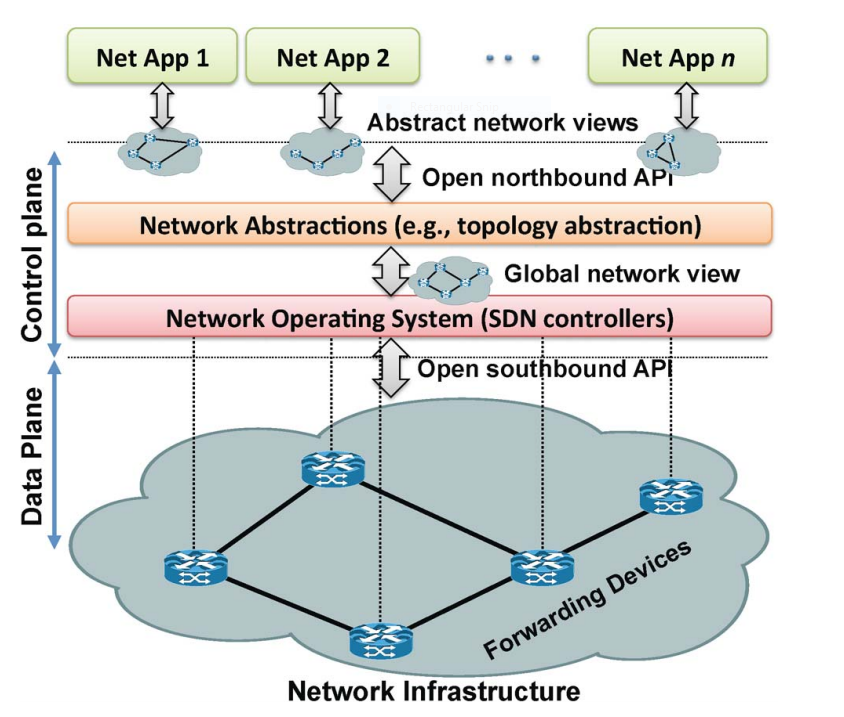
\includegraphics[width=0.75\linewidth]{fig/sdn-infrastructure.png}
	\caption{Kiến trúc của SDN \cite{11-Kreutz}}
	\label{fig:sdn-infrastructure}
\end{figure}

Openflow \cite{13-McKeown} được đề xuất để tiêu chuẩn giao tiếp giữa các switch và controller trong kiến trúc SDN \cite{14-Lara}. Các tác giả nhận định rằng, thật khó để cộng đồng nghiên cứu mạng có thể kiểm tra ý tưởng mới ở các phần cứng hiện tại. Việc này diễn ra bởi vì mã nguồn của phần mềm chạy trên các switch không thể được tùy chỉnh và các kiến trúc mạng thì luôn cố định, dẫn tới những ý tưởng mạng mới không thể được kiểm tra trên những cài đặt lưu lượng thực tế. Bằng việc xác định các đặc trưng thông thường trên những bảng luồng trong các switch Ethernet, các tác giả đã cung cấp cách điều khiển switch mà không cần quan tâm đến mã nguồn trên các thiết bị đó.
	
Openflow lần đầu được triển khai trong khuôn viên mạng đại học \cite{13-McKeown}. Ngày nay, có ít nhất 9 trường đại học ở Hoa Kỳ triển khai công nghệ này. Mục đích của Openflow là cung cấp nền tảng mà có thể cho phép các nhà nghiên cứu chạy thử nghiệm những sản phẩm mạng. Tuy nhiên, SDN và Openflow được gắn kết như chiến lược để gia tăng chức năng chức năng của mạng trong khi giảm thiểu chi phí và độ phức tạp phần cứng. Openflow Networking Foundation (ONF) được thành lập vào năm 2011 bởi Deutsche Telekom, Facebook, Google, Microsoft, Verizon và Yahoo để khuyến khích áp dụng mạng dựa trên SDN và Openflow. Hiện tại, ONF có hơn 95 thành viên bào gồm thành viên sáng lập.

Bảng \ref{tab:ofswitch-company} liệt kê một số công ty cung cấp Openflow switch trên thị trường.

\begin{table}[ht!]
	\centering
	\begin{tabular}{|l|l|}
		\hline
		\multicolumn{1}{|c|}{\textbf{Switch company}} &
		\multicolumn{1}{c|}{\textbf{Series}} \\ \hline
		Arista &
		\begin{tabular}[c]{@{}l@{}}Arista   extensible modular operating system (EOS),\\  Arista 7124FX application switch\end{tabular} \\ \hline
		Ciena          & Ciena   Coredirector running firmware version 6.1.1 \\ \hline
		Cisco          & Cisco   cat6k, catalyst 3750, 6500 series           \\ \hline
		HP &
		\begin{tabular}[c]{@{}l@{}}HP   procurve series- 5400 zl, 8200 zl, 6200 yl, \\ 3500 yl, 6600\end{tabular} \\ \hline
		NEC            & NEC   IP8800                                        \\ \hline
		Open   vSwitch & Software   switch.                                  \\ \hline
	\end{tabular}
\caption{Một số công ty cung cấp OpenFlow Switch}
\label{tab:ofswitch-company}
\end{table}

Trong khuôn khổ của khóa luận này, Open vSwitch sẽ được sử dụng là một thành phần chính trong triển khai SDN, được giới thiệu chi tiết trong mục \ref{sec:openvswtich}.

\subsection{Open vSwitch}
\label{sec:openvswtich}

\subsubsection{Open vSwitch (OVS) là gì?}

Open vSwitch là switch phần mềm đa lớp bản quyền mã nguồn mở Apache 2. Mục tiêu là để triển khai một nền tảng sản phẩm switch chất lượng hỗ trợ các giao diện quản lý tiêu chuẩn và mở ra chức năng chuyển tiếp để mở rộng và kiểm soát bằng lập trình.

OVS rất thích hợp với chức năng như một switch ảo trong môi trường máy ảo. Ngoài việc hiển thị các giao diện điều khiển và hiển thị tiêu chuẩn cho lớp mạng ảo, nó còn được thiết kế để hỗ trợ phân phối trên nhiều máy chủ vật lý. OVS hỗ trợ nhiều công nghệ ảo hóa dựa trên Linux bao gồm Xen/XenServer, KVM và Virtualbox. Hình \ref{fig:ovs} thể hiện kiến trúc tổng quan và chức năng của OVS.

\begin{figure}[ht!]
	\centering
	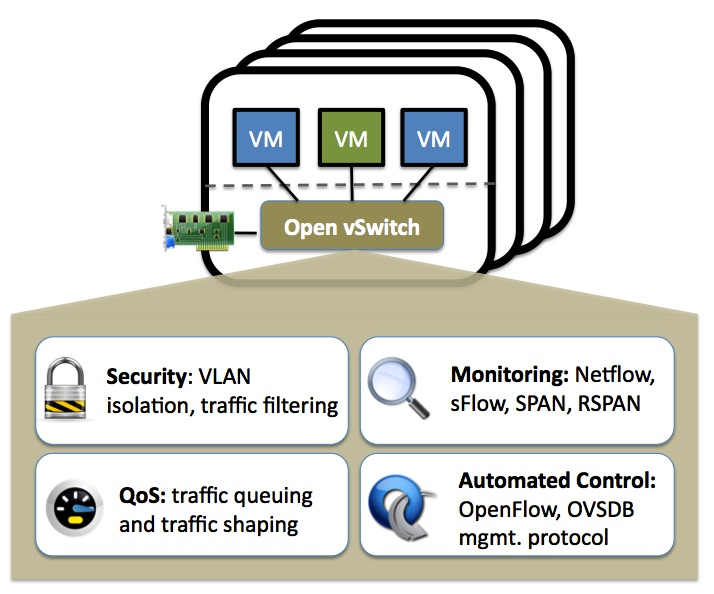
\includegraphics[width=0.5\linewidth]{fig/ovs.png}
	\caption{Kiến trúc tổng quan và chức năng của OVS \cite{16-openvswitch}}
	\label{fig:ovs}
\end{figure}

\subsection{Vai trò của SDN controller}

\subsubsection{Tổng quan}

Dựa theo các định nghĩa đã được đưa ra, SDN controller là hệ quả của việc tách rời Data plane và Control plane trong hệ thống mạng. Nó có vai trò trung tập điều khiển tất cả các hoạt động của mạng bằng việc điều khiển các switch và router thông qua flow-table. Nói cách khác, SDN controller như là bộ não của toàn bộ hệ thống. Để có thể giao tiếp với các thiết bị mạng, SDN controller sử dụng một giao thức chuẩn là Openflow như đã đề cập tại mục \ref{sec:sdn}. Hình \ref{fig:sdn-infrastructure} cho thấy, SDN controller như một cầu nối giữa các thiết bị mạng và các ứng dụng ở phần trên.

Hiện nay có rất nhiều phần mềm hay framework hỗ trợ việc lập trình SDN controller như OpenDaylight, ONOS, POX, Ryu, vv. Trong khuôn khổ của dự án này, Ryu framework được sử dụng như thành phần chính để lập trình và thực thi SDN controller, được giới thiệu chi tiết bên dưới mục "Framework RYU".

\subsubsection{Framework RYU}
\label{sec:ryu}

Theo \cite{17-Asadollahi}, Ryu Controller là một dự án mã nguồn mở dưới giấy phép của Apache 2.0, được viết hoàn toàn dựa trên Python, được hỗ trợ và triển khai bởi trung tâm dữ liệu đám mây NTT. Phần mã nguồn chính có thể được tìm thấy trên Github, được cung cấp và hỗ trợ bởi Open Ryu Community. Nó hỗ trợ quản trị mạng NETCONF và OF-config, còn được biết đến là Openflow. Ryu đã được kiểm định với OVS switch, Hewlett Packard, IBM và NEC. Hiện tại nó đang hỗ trợ đến phiên bản Openflow 1.5.

Cũng như các SDN controller khác, Ryu cũng tạo ra các gói tin Openflow, quản lý các sự kiện liên quan tới những gói tin đến và đi. Nó còn có một danh sách phong phú các thư viện hỗ trợ xử lý hoạt động của các gói tin. Về hỗ trợ các giao thức southbound, 	Ryu hợp tác với các giao thức như Xflow (Netflow và Sflow), OF-config, NETCONF, Open vSwitch Database Protocol, vv, VLAN và GRE cũng được hỗ trợ bởi những thư viện gói tin của Ryu.

\section{Học máy (Machine Learning)}

\subsection{Học máy là gì?}

Theo A.Dey \cite{18-Dey} trích dẫn, học máy được dùng để dạy máy móc cách để xử lý dữ liệu hiệu quả hơn. Đôi khi, sau khi xem xét dữ liệu, chúng ta không thể giải thích được mẫu hoặc trích xuất thông tin từ chúng. Trong trường hợp này, chúng ta có thể áp dụng học máy. Với vô số tập dữ liệu (dataset) hiện có, nhu cầu về học máy ngày càng tăng. Rất nhiều ngành công nghiệp từ dược liệu cho đến quân sự đều ứng dụng học máy để trích xuất thông tin liên quan từ dữ liệu. Công việc chính của học máy là học từ dữ liệu. Có rất nhiều nghiên cứu đã tìm ra được cách để máy móc có thể học từ chính chúng \cite{19-Welling}, \cite{20-Bowles}. Có rất nhiều nhà toán học và lập trình viên ứng dụng nhiều hướng tiếp cận để tìm ra giải pháp cho vấn đề này. Một vài trong số chúng được biểu thị trong hình \ref{fig:ml-algo}.

\begin{figure}[ht!]
	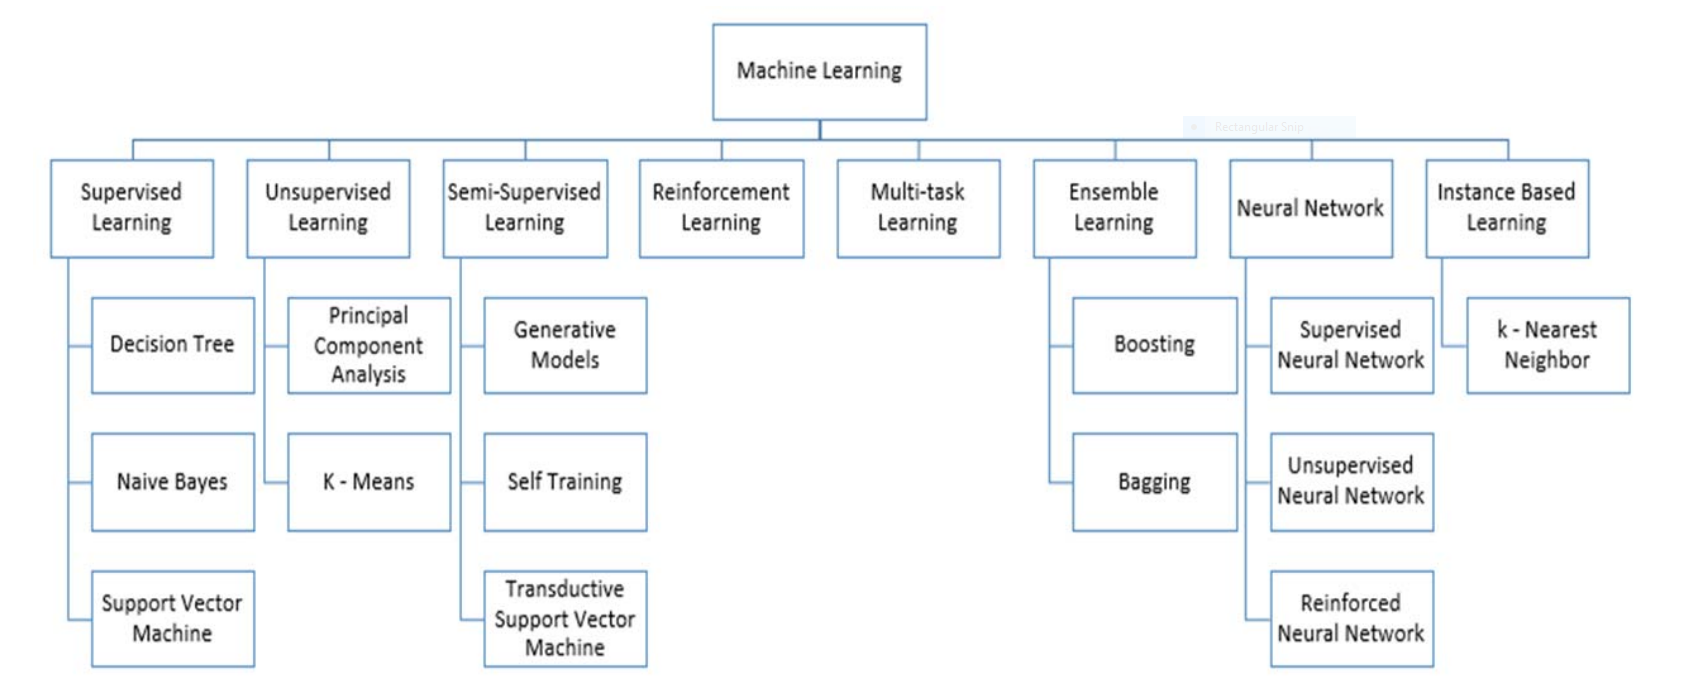
\includegraphics[width=\linewidth]{fig/ml-algo.png}
	\caption{Một số giải thuật học máy \cite{18-Dey}}
	\label{fig:ml-algo}
\end{figure}

\subsection{Mô hình học máy}

Theo như hình \ref{fig:ml-algo}, học máy được phân ra thành rất nhiều loại như Supervised learning (học có giám sát), Unsupervised learning (học không có giám sát), Semi-supervised learning (học bán giám sát), vv. Trong khuôn khổ của khóa luận này, tôi chỉ giới thiệu một số giải thuật là Support Vector Machine, Naïve Bayes, Decision Tree và Random Forest trong nhóm Học có giám sát, vì đây là các giải thuật được tôi áp dụng vào khóa luận.

\subsubsection{Học có giám sát}

Các thuật toán học có giám sát là những thuật toán cần sự hỗ trợ từ bên trong. Đầu vào của dữ liệu cần chia ra thành tập huấn luyện (train set) và tập kiểm tra (test set). Train set có giá trị đầu ra, thứ cần được dự đoán hoặc phân loại. Tất cả các thuật toán đều được học hình mẫu từ train set và sau đó vận dụng chúng vào test set để đánh giá \cite{21-Kotsiantis}. Giải thuật học có giám sát được biểu thị trong hình \ref{fig:supervised-ml}.

\begin{figure}[ht!]
	\centering
	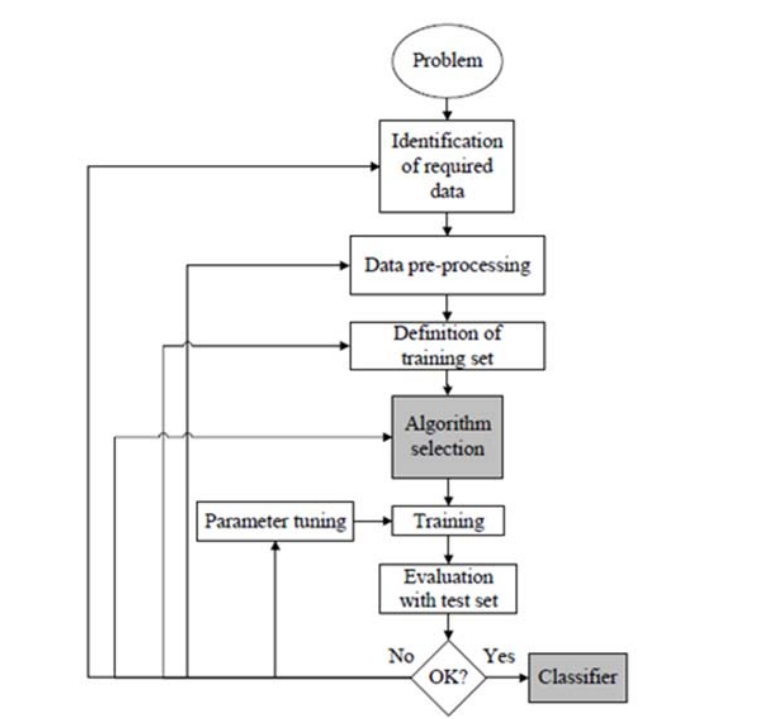
\includegraphics[width=0.6\linewidth]{fig/supervised-ml.png}
	\caption{Giải thuật học máy có giám sát \cite{18-Dey}}
	\label{fig:supervised-ml}
\end{figure} 

\subsubsection{Support Vector Machine}

Một kỹ thuật học máy state-of-the-art được sử dụng rộng rãi là Support Vector Machine (SVM). Nó được dùng chủ yếu trong bài toán phân loại. SVM hoạt động dựa trên nguyên lý của tính toán biên. Các biên được vẽ sao cho khoảng cách giữa biên đến các lớp là lớp nhất và vì vậy giảm thiểu sai số phân loại. Mô tả SVM được biểu thị trong hình \ref{fig:svm-overview}.

\begin{figure}[ht!]
	\centering
	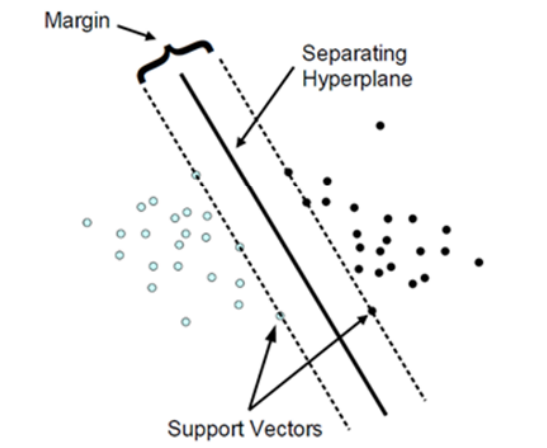
\includegraphics[width=0.5\linewidth]{fig/svm-overview.png}
	\caption{Mô tả mô hình SVM \cite{18-Dey}}
	\label{fig:svm-overview}
\end{figure}

\subsubsection{Naïve Bayes}

Naïve Bayes được áp dụng chủ yếu trong lĩnh vực phân loại văn bản. Nó được sử dụng chủ yếu cho việc phân cụm và phân lớp. Kiến trúc cơ bản của Naïve Bayes phụ thuộc vào xác suất có điều kiện. Nó tạo ra cây dựa trên xác suất xảy ra của chúng. Những cây này được gọi là Bayesian Network. Ví dụ cho Bayesian Network được biểu thị trong hình \ref{fig:naive-bayes-example}.

\begin{figure}[ht!]
	\centering
	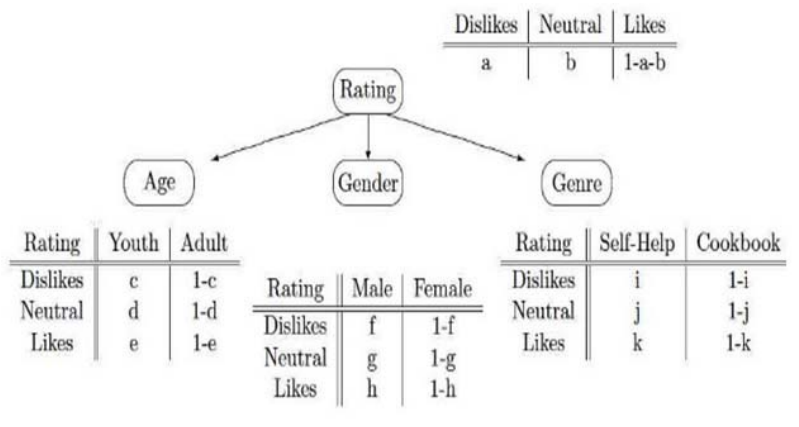
\includegraphics[width=0.75\linewidth]{fig/naive-bayes-example.png}
	\caption{Một ví dụ về Bayesian Network \cite{18-Dey}}
	\label{fig:naive-bayes-example}
\end{figure}

\subsubsection{Decision Tree}

Decision trees (những cây quyết định) là những loại cây gom nhóm các thuộc tính dựa trên giá trị của chúng. Decision tree được sử dụng chủ yếu cho việc phân lớp. Môi cây chứa nhiều nút và nhiều nhánh. Mỗi nút biểu diễn cho những thuộc tính trong một nhóm để phân lớp và mỗi nhánh biểu diễn một giá trị  mà nút đó có thể lấy. Một ví dụ cho Decision tree trong hình \ref{fig:decision-tree-example}.

\begin{figure}[ht!]
	\centering
	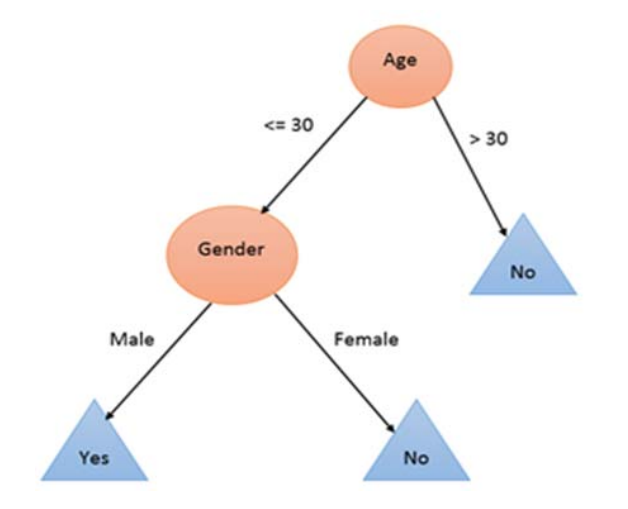
\includegraphics[width=0.6\linewidth]{fig/decision-tree-example.png}
	\caption{Một ví dụ cho Decision Tree}
	\label{fig:decision-tree-example}
\end{figure}

\subsubsection{Random Forest}

Random forest được đề xuất lần đầu bởi Leo Breiman từ đại học California vào năm 2001. Nó kết hợp nhiều máy phân lớp đơn giản (các cây quyết định) độc lập với nhau. Kết quả của phân lớp của một mẫu được đưa ra bởi nhiều cây quyết đinh, kết quả cuối cùng sẽ được bình chọn dựa trên kết quả của các cây quyết định này \cite{70-Parmar}.Toàn bộ quy trình phân lớp dựa trên Random Forest được biểu diễn như trong hình \ref{fig:random-forest-example}.

\begin{figure}[ht!]
	\centering
	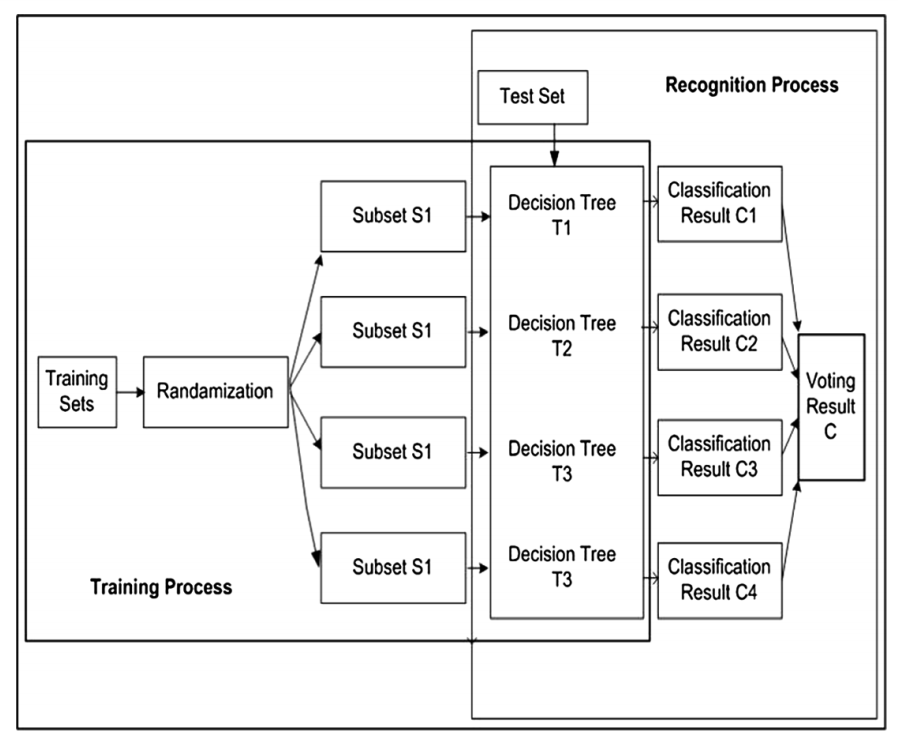
\includegraphics[width=0.75\linewidth]{fig/random-forest-example.png}
	\caption{Quá trình máy phân lớp  Random  forest}
	\label{fig:random-forest-example}
\end{figure}

\subsection{Thư viện scikit-learn}

Scikit-learn là thư viện cung cấp sẵn một lượng lớn các giải thuật học máy có giám sát và không có giám sát thông qua giao diện lập trình Python.

Đây là thư viện mã nguồn mở, giấy phép cấp bởi BSD và được phân phối sẵn trên nhiều nền tảng hệ điều hành Linux.

Scikit-learn được phát triển lần đầu bởi David Cournapeau như một dự án mùa hè tại Google năm 2007. Sau đó Matthieu Brucher tham gia dự án và bắt đầu sử dụng thư viện này như một phần trong luận văn của anh ấy. Năm 2010, INRIA tham gia và lần đầu xuất bản phiên bản đầu tiên (v0.1 beta) vào cuối tháng 1 năm 2010. Dự án hiện tại có trên 30 nhà phát triển đóng góp và được tài trợ trả phí từ INRIA, Google, Tinyclues và Python software foundation.

\section{Học sâu (Deep learning)}

\subsection{Học sâu là gì}

Theo X. Du và các cộng sự \cite{25-Du}, học sâu trong quá khứ được phát triển từ mạng nơ-ron nhân tạo, và bây giờ nó trở nhành một lĩnh vực thịnh hành của học máy. Nghiên cứu về mạng nơ-ron nhân tạo bắt đầu từ những năm 1940. McCulloch và các cộng sự \cite{26-McCulloch} đã đề xuất mô hình McCulloch-Pitts với việc phân tích và tổng hợp những nét đặc trưng của mạng nơ-ron. Khái niệm học sâu được đưa ra lần đầu vào năm 2006. Sau đó, học sâu vẫn tiếp tục được phát triển mạnh. Hiện tại, có rất nhiều tên tuổi nổi bật như Geoffrey Hinton, Yoshua Bengio, Yann LeCun và Andrew Ng. Họ là những người dẫn đầu về hướng nghiên cứu học sâu. 

Một số doanh nghiệp, ví dụ như Google và Facebook đã có rất nhiều nghiên cứu đạt được thành công và áp dụng trong nhiều lĩnh vực khác nhau. Đơn cử như Google’s AlphaGo đã đánh bại Lee Sedol – kỳ thủ cờ vây chuyên nghiệp người Hàn Quốc, cho thấy khả năng học rất mạnh của học sâu. Hơn nữa, Google’s DeepDream và một phần mềm tuyệt vời, thứ không chỉ phân loại hình ảnh mà còn tạo ra được những hình vẽ nhân tạo kỳ lạ dựa trên chính kiến thức của nó. Bên cạnh đó, Facebook với DeepText – một kỹ thuật hiểu văn bản dựa trên học sâu, có thể phân loại một lượng dữ liệu khổng lồ, cung cấp dịch vụ phản hồi sau khi xác định những đoạn trò chuyện của người dùng và xóa các đoạn thư spam.

\subsection{Mô hình học sâu}

\subsubsection{Khái niệm và phân loại}

\textit{Mạng nơ-ron - Neural Network}

Mạng nơ-ron (hay mạng nơ-ron nhân tạo hay ANN) được kế thừa từ khái niệm nơ-rơn sinh học. Một nơ-rơn như một cấu trúc trong não. Để hiểu được mạng nơ-ron, người ta cần phải hiểu cách hoạt động của nơ-ron. Một nơ-ron bao gồm 4 phần chính là dendrites, nucleus, soma và axon (Hình \ref{fig:bio-nn}). 

\begin{figure}[ht!]
	\centering
	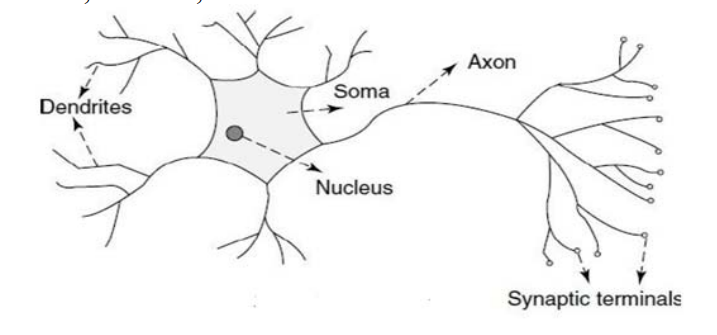
\includegraphics[width=0.75\linewidth]{fig/bio-nn.png}
	\caption{Mạng nơ-ron sinh học}
	\label{fig:bio-nn}
\end{figure}

Các dendrite nhận tín hiệu điện. Soma xử lý tín hiệu điện. Đầu ra của quá trình được vận chuyển bởi axon đển cổng dendrite nơi mà đầu ra được gửi tiếp đến nơ-ron tiếp theo. Necleus là trái tim của nơ-ron. Kết nối bên trong nơ-ron được gọi là mạng nơ-ron nơi mà các xung điện di chuyển khắp não.

Một mạng nơ-ron nhân tạo cũng hoạt động tương tự. Nó hoạt động với 3 tầng. Tầng đầu vào (input) nhận dữ liệu đầu vào (tương tự dendrite). Những tầng ẩn thì xử lý dữ liệu (tương tự soma và axon). Cuối cùng, tầng đầu ra (output) gửi kết quả đã được tính toán (tương tự dendrite terminal). Cấu trúc ví dụ của mạng nơ-ron nhân tạo được biểu thị trong hình \ref{fig:cs-nn}

\begin{figure}[h]
	\centering
	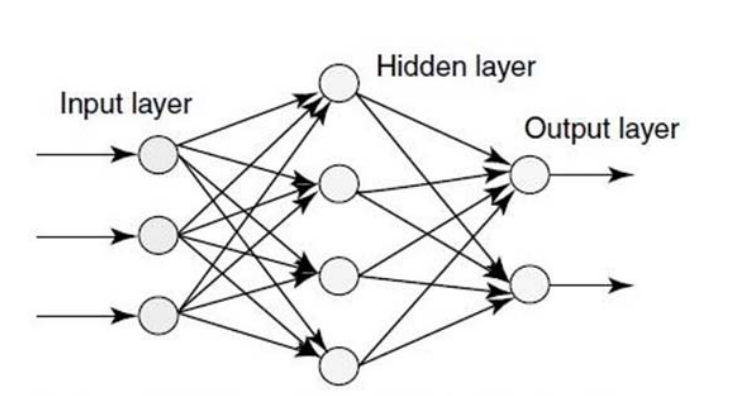
\includegraphics[width=0.75\linewidth]{fig/cs-nn.png}
	\caption{Mạng nơ-ron nhân tạo}
	\label{fig:cs-nn}
\end{figure}

Theo Shrestha và các cộng sự \cite{62-Shrestha}, mạng nơ-ron nhân có thể được chia ra thành các loại sau:

\begin{itemize}
	\item[--] Mạng nơ-ron suy luận tiến (Feedforward Neural Network)
	\item[--] Mạng nơ-ron hồi quy (Recurrent Neural Network (RNN))
	\item[--] Mạng chức năng cơ sở xuyên tâm (Radial Basis Function Neural Network)
	\item[--] Mạng nơ-ron ánh xạ đặc trưng tự tổ chức (Kohonen Self Organizing Neural Network)
	\item[--] Mạng nơ-ron mô-đun
\end{itemize}

Trong mạng nơ-ron suy luận tiến, những luồng thông tin chỉ đi theo 1 chiều từ  lớp đầu vào đến lớp đầu ra (đi qua các nút ẩn nếu có). Chúng không có tạo thành bất cứ vòng lặp hay luận lùi. Hình \ref{fig:feed-forward-nn} biểu thị một triển khai cụ thể của mạng nơ-ron suy tiến đa lớp với các giá trị và các hàm được tính toán theo chiều tiến. Z là tổng trọng số của các đầu vào và y biểu diễn một hàm không tuyến tính f của Z ở mỗi lớp. W biểu diễn cho những trọng số giữa 2 đơn vị trong những lớp liền kề biểu diễn bởi ký tự chỉ số dưới và b biểu diễn cho giá trị sai khác của đơn vị.

\begin{figure}[ht!]
	\centering
	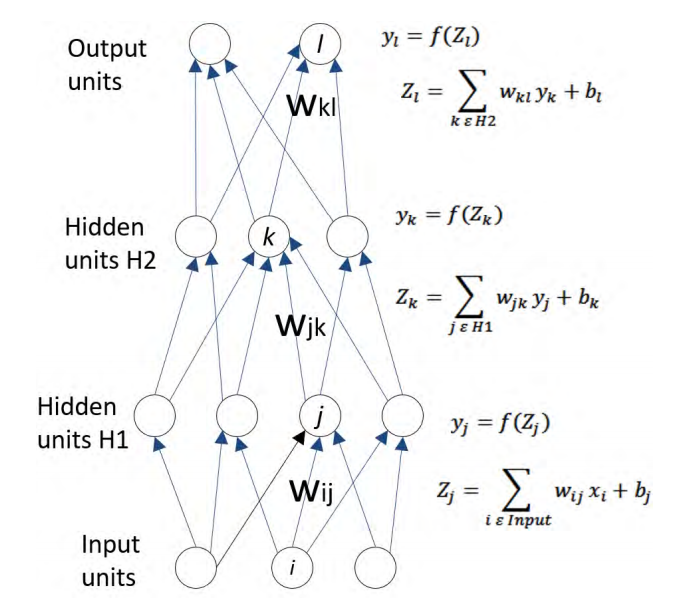
\includegraphics[width=0.6\linewidth]{fig/feed-forward-nn.png}
	\caption{Mạng nơ-ron suy luận tiến \cite{62-Shrestha}}
	\label{fig:feed-forward-nn}
\end{figure}

Không giống như mạng nơ-ron suy luận tiến, việc xử lý đơn vị trong RNN có vòng lặp. Đầu ra của lớp trước trở thành đầu vào cho lớp sau, thứ đơn thuần chỉ là 1 lớp trong mạng, vì vậy chính đầu ra của lớp cũng trở thành chính đầu vào của nó biểu diễn một vòng tự lặp. Điều này cho phép mạng có ký tức về những trạng thái trước đó và sử dụng nó để ảnh hướng lên đầu ra hiện tại. Một lợi thế lớn của đặc điểm này so với mạng nơ-ron suy tiến là RNN có thể nhận chuỗi đầu vào và trả về chuỗi đầu ra, vì vậy nó rất hữu ích cho các ứng dụng cần xử lý đầu vào dạng chuỗi theo thời gian như nhận diện giọng nói, phân loại từng khung hình của video, vv. Hình \ref{fig:rnn} biểu diễn một triển khai của RNN. Trong đó \(x^t\) biểu diễn cho đầu vào tại thời điểm t. U, V và W là các  tham số học được chia sẽ bởi tất cả bước. \(O_t\) là đầu ra tại thời điểm t. \(S_t\) biểu diễn trạng thái tại thời điểm t.

\begin{figure}[ht!]
	\centering
	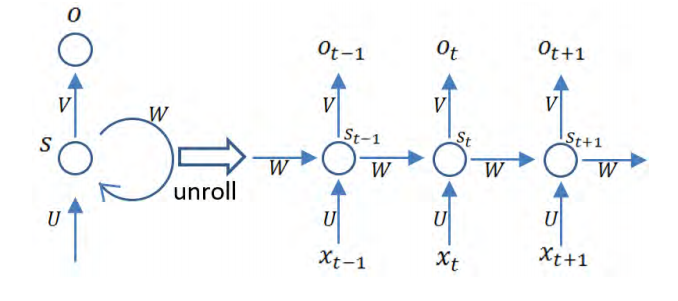
\includegraphics[width=0.75\linewidth]{fig/rnn.png}
	\caption{Mạng nơ-ron hồi quy \cite{62-Shrestha}}
	\label{fig:rnn}
\end{figure}

Mạng chức năng cơ sở xuyên tâm được dùng trong phân lớp, xấp xỉ hàm, những vấn đề dự doán theo thời gian, vv.

Mạng nơ-ron ánh xạ đặc trưng tự tổ chức có thể tự tổ chức mô hình mạng dựa trên dữ liệu đầu vào bằng việc học không giám sát.

Mạng nơ-ron mô-đun tách một mạng lớn thành các mô-đun mạng nơ-ron nhỏ độc lập. Những mạng nhỏ hơn giải quyết công việc khác nhau và sau đó kết hợp tại một điểm đầu ra của toàn bộ mạng.

\subsubsection{Một số khái niệm về các hàm huấn luyện}

\textit{Hàm kích hoạt (Activation function)}

Theo \cite{63-Nwankpa}, những hàm kích hoạt là những hàm dùng trong mạng nơ-ron để tính toán tổng trọng số của đầu vào và những sai khác (bias), thứ quyết định nơ-ron được thực hiện hay không. Nó thao tác với dữ liệu thông qua quá trình gradient thường là giảm gradient và sau đó sinh ra kết quả cho mạng nơ-ron mà có chứa tham số cho dữ liệu. Hàm kích hoạt có thể tuyến tính hoặc không tuyến tính tùy thuộc vào hàm mà nó  biểu diễn và được dùng để điều khiển đầu ra cho mạng nơ-ron.  Một số hàm kích hoạt biểu diễn trong công thức (\ref{eq:softmax}) và (\ref{eq:relu}).

\begin{itemize}
	\item[--] Hàm  Softmax: 
		\begin{gather}
		\label{eq:softmax}
			f(x) = \frac{exp(x_i)}{\sum_{j} exp(x_j)}
		\end{gather} 
	\item[--] Hàm ReLU: 
		\begin{gather}
		\label{eq:relu}
			f(x) = max(0, x)
		\end{gather}
\end{itemize}

\textit{Hàm mất mát (Loss function)}

Hàm mất mát đơn giản là hàm dùng để đánh giá mức độ tốt của mô hình giải thuật. Nếu dự đoán tốt hàm sẽ cho ra giá trị thấp, ngược lại hàm cho ra giá trị cao. Công thức của hàm mất mát Categorical Cross Entroy biểu diễn ở công thức (\ref{eq:loss_cce}).

\begin{gather}
\label{eq:loss_cce}
	Loss = - \sum_{i=1}^{output size} y_i \cdot log \hat{y}_i
\end{gather}

\subsection{Thư viện Tensorflow và Keras}

Tensorflow hiện nay là bộ thư viện học sâu nổi tiếng nhất được phát triển bởi Google. Nó lần đầu tiên được công bố vào cuối năm 2015, trong khi phiên bản ổn định đầu tiên ra đời năm 2017. Tensorflow là thư viện mã nguồn mở dưới giấy phép của Apache Opensource. Người ta có thể sử dụng, tinh chỉnh, và phân phối lại phiên bản tinh chỉnh mà không cần phải trả một khoản nào cho Google.

Keras là một thư viện mã nguồn dưới bản quyền MIT. Keras cung cấp một API ở mức cao, nằm trên các thư viện học sâu như Tensorflow, Theano, CNTK với mục tiêu giúp đơn giản hóa việc tiếp cận nền tảng học sâu. Keras được xây dựng với mục đích cung cấp giao diện thân thiện, mô-đun hóa, và dễ mở rộng.

Năm 2017, Google’s Tensorflow team quyết định hỗ trợ Keras nằm trực tiếp trong phần nhân của thư viện tensorflow.
